\subsection{矩阵乘法算法对 Cache 命中率的影响}

前面的实验主要从 Cache 参数角度分析了命中率变化，包括 Cache 容量、块大小、相联度、替换算法和矩阵规模等因素。但对于矩阵乘法这类数据密集型程序而言，程序本身的访存模式同样会显著影响 Cache 命中率。因此，本节进一步比较普通三重循环矩阵乘法和分块矩阵乘法在不同 Cache 容量下的命中率差异。

\subsubsection{实验设计}

本组实验选取矩阵规模为 $N=128$ 的访存 trace 作为分析对象，比较两种矩阵乘法实现方式：

\begin{itemize}
    \item 普通 IJK 矩阵乘法：直接使用三重循环计算矩阵乘法；
    \item 分块矩阵乘法：将矩阵划分为若干小块，使局部计算所需的数据尽可能保留在 Cache 中。
\end{itemize}

实验固定参数如下：

\begin{itemize}
    \item 矩阵规模：$N=128$；
    \item Cache 块大小：64B；
    \item 映射方式：4 路组相联；
    \item 替换算法：LRU；
    \item Cache 容量：4KB、8KB、16KB、32KB、64KB、128KB。
\end{itemize}

本实验分别使用普通矩阵乘法生成的 \texttt{trace\_n128.log} 和分块矩阵乘法生成的 \texttt{trace\_blocked\_n128.log} 作为输入，通过自行编写的 Cache 模拟器统计不同容量下的 Cache 命中率。

\subsubsection{普通矩阵乘法的访存特征}

普通 IJK 矩阵乘法的核心形式如下：

\begin{lstlisting}[language=C, caption={普通 IJK 矩阵乘法}]
for (int i = 0; i < N; i++) {
    for (int j = 0; j < N; j++) {
        for (int k = 0; k < N; k++) {
            C[i][j] += A[i][k] * B[k][j];
        }
    }
}
\end{lstlisting}

在该实现中，矩阵 $A$ 的访问形式为 $A[i][k]$，随着 $k$ 增加，访问的是同一行中的连续元素，因此具有较好的空间局部性。矩阵 $C[i][j]$ 在内层循环中被反复累加，因此具有一定的时间局部性。

但是，矩阵 $B$ 的访问形式为 $B[k][j]$。当 $k$ 增加时，程序访问的是矩阵 $B$ 的同一列，内存地址之间的跨度为一整行。对于 $N=128$ 的 int 型矩阵，一行大小为：

\[
128 \times 4B = 512B
\]

这意味着矩阵 $B$ 的连续访问步长为 512B，远大于本实验中的 Cache 块大小 64B。因此，普通 IJK 矩阵乘法难以充分利用矩阵 $B$ 的空间局部性，容易造成大量 Cache Miss。

\subsubsection{分块矩阵乘法的优化思想}

分块矩阵乘法的核心思想是将原矩阵划分为若干较小的子块，每次只在局部子块上进行计算。其基本形式如下：

\begin{lstlisting}[language=C, caption={分块矩阵乘法}]
for (int ii = 0; ii < N; ii += BS) {
    for (int jj = 0; jj < N; jj += BS) {
        for (int kk = 0; kk < N; kk += BS) {
            for (int i = ii; i < ii + BS; i++) {
                for (int j = jj; j < jj + BS; j++) {
                    for (int k = kk; k < kk + BS; k++) {
                        C[i][j] += A[i][k] * B[k][j];
                    }
                }
            }
        }
    }
}
\end{lstlisting}

其中，$BS$ 表示分块大小。与普通 IJK 算法相比，分块算法并没有改变矩阵乘法的数学结果，而是改变了程序访问内存的顺序。通过在一个较小的数据块内集中完成计算，分块算法可以提高数据被重复利用的概率，使矩阵 $A$、$B$ 和 $C$ 的局部子块尽可能停留在 Cache 中，从而减少容量缺失和替换缺失。

\subsubsection{实验结果}\begin{table}[H]
\centering
\caption{相联度对 Cache 命中率的影响}
\begin{tabular}{c|c|c}
\hline
Cache大小 & IJK算法命中率 & 分块算法命中率\\
\hline
4KB & 49.75& 96.69\\
8KB & 49.75 & 96.69 \\
16KB & 49.76& 98.99\\
32KB &49.77 & 99.74\\
64KB &97.27 &99.77 \\
128 & 99.85&99.87\\
\hline
\end{tabular}
\end{table}

实验结果数据绘制如图 \ref{fig:algorithm_impact} 所示。图中红色曲线表示普通 IJK 矩阵乘法，绿色曲线表示分块矩阵乘法。

\begin{figure}[H]
    \centering
    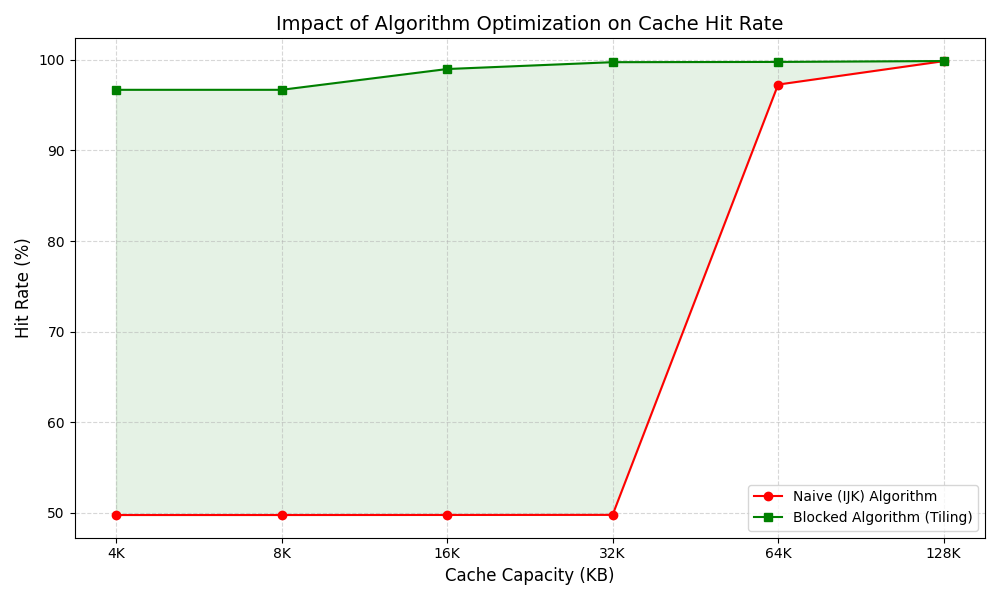
\includegraphics[width=0.82\textwidth]{figure/algorithm_impact.png}
    \caption{矩阵乘法算法对 Cache 命中率的影响}
    \label{fig:algorithm_impact}
\end{figure}

从图中可以看出，在 Cache 容量较小时，普通 IJK 算法的命中率长期维持在约 $50\%$ 左右；而分块矩阵乘法即使在 4KB、8KB 等较小 Cache 容量下，也能保持较高命中率，约在 $96\%$ 以上。随着 Cache 容量增大，分块算法的命中率进一步接近 $100\%$。

当 Cache 容量达到 64KB 及以上时，普通 IJK 算法的命中率也出现明显提升。这与前文 Cache 容量实验中的现象一致：当 Cache 容量达到单个 $128 \times 128$ int 型矩阵大小附近时，普通算法中的活跃数据可以被更好地缓存，因此命中率发生跃升。

\subsubsection{实验现象与分析}

本组实验最明显的现象是：在小容量 Cache 下，分块矩阵乘法远优于普通 IJK 矩阵乘法。普通 IJK 算法在 4KB 到 32KB 的 Cache 容量范围内命中率基本维持在约 $50\%$，说明此时 Cache 容量不足以容纳主要活跃数据，同时矩阵 $B$ 的跨行访问导致空间局部性利用较差。

相比之下，分块矩阵乘法通过限制每次计算所涉及的数据范围，使程序在短时间内反复访问同一批矩阵子块。这样一来，已经装入 Cache 的数据块在被替换之前可以被多次使用，从而显著提高时间局部性和空间局部性的利用效率。因此，即使 Cache 容量只有 4KB 或 8KB，分块算法仍然能够维持较高命中率。

从程序访存模式看，普通 IJK 算法的主要问题在于矩阵 $B[k][j]$ 的按列访问。每次访问相邻的 $k$ 值时，地址跨越 512B，远大于 64B 的 Cache 块大小，因此一个 Cache 块被加载后，其中相邻数据很难被立即利用。分块算法则通过固定一小段 $kk$ 范围，使矩阵 $B$ 的局部块在一段时间内被反复访问，从而提高了 Cache 块中数据的利用率。

此外，图中也显示出：随着 Cache 容量增大，普通 IJK 算法和分块算法之间的差距逐渐缩小。当 Cache 容量达到 128KB 时，两种算法的命中率都接近 $100\%$。这说明当 Cache 容量足够大时，硬件容量本身已经能够覆盖大部分活跃工作集，代码访存优化带来的额外收益会减小；而当 Cache 容量较小时，分块优化对命中率的提升最为明显。

\subsubsection{实验总结}

通过普通 IJK 矩阵乘法和分块矩阵乘法的对比可以看出，Cache 命中率不仅取决于 Cache 容量、块大小、相联度和替换算法，也强烈依赖于程序本身的访存模式。

普通矩阵乘法由于矩阵 $B$ 的按列访问，难以充分利用 Cache 块内的空间局部性，因此在小容量 Cache 下命中率较低。分块矩阵乘法通过限制局部计算的数据范围，使矩阵子块能够在 Cache 中被重复利用，从而显著提高命中率。

因此，对于矩阵乘法这类数据密集型程序，单纯依靠增大 Cache 容量并不是唯一优化方式。通过分块等程序级优化方法改善访存局部性，可以在 Cache 容量较小的情况下显著减少 Cache Miss，提高程序的访存效率。